\clearpage % clear the prior chapter's page

\chapter{Supplement to "pH-dependent structural dynamics of the glutamate-GABA antiporter GadC"} \label{app:gadc_supp}
%\vspace{-7mm}
%\bigskip

This Appendix contains supplementary information for Chapter \ref{ch:gadc}.

\begin{figure}[h]
\centering
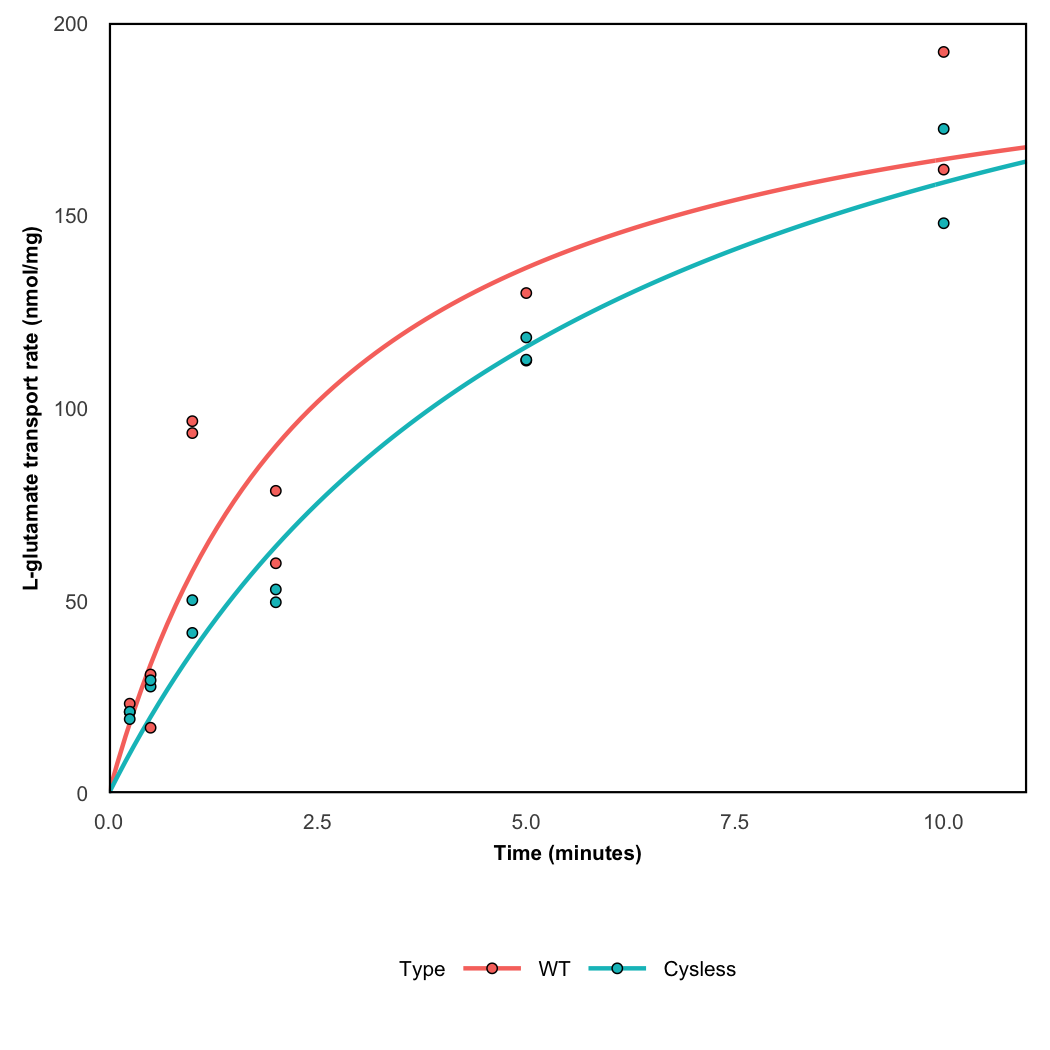
\includegraphics[width=3.5in]{Figures/gadc_supp_time_transport.png}
\caption[Time-dependent glutamate transport by wildtype and cysless GadC reconstituted into proteoliposomes filled with GABA.]{Time-dependent glutamate transport by wildtype and cysless GadC reconstituted into proteoliposomes filled with \SI{5}{mM} GABA.}
\label{fig:gadc_supp_time_transport}
\end{figure}

\begin{figure}[h]
\centering
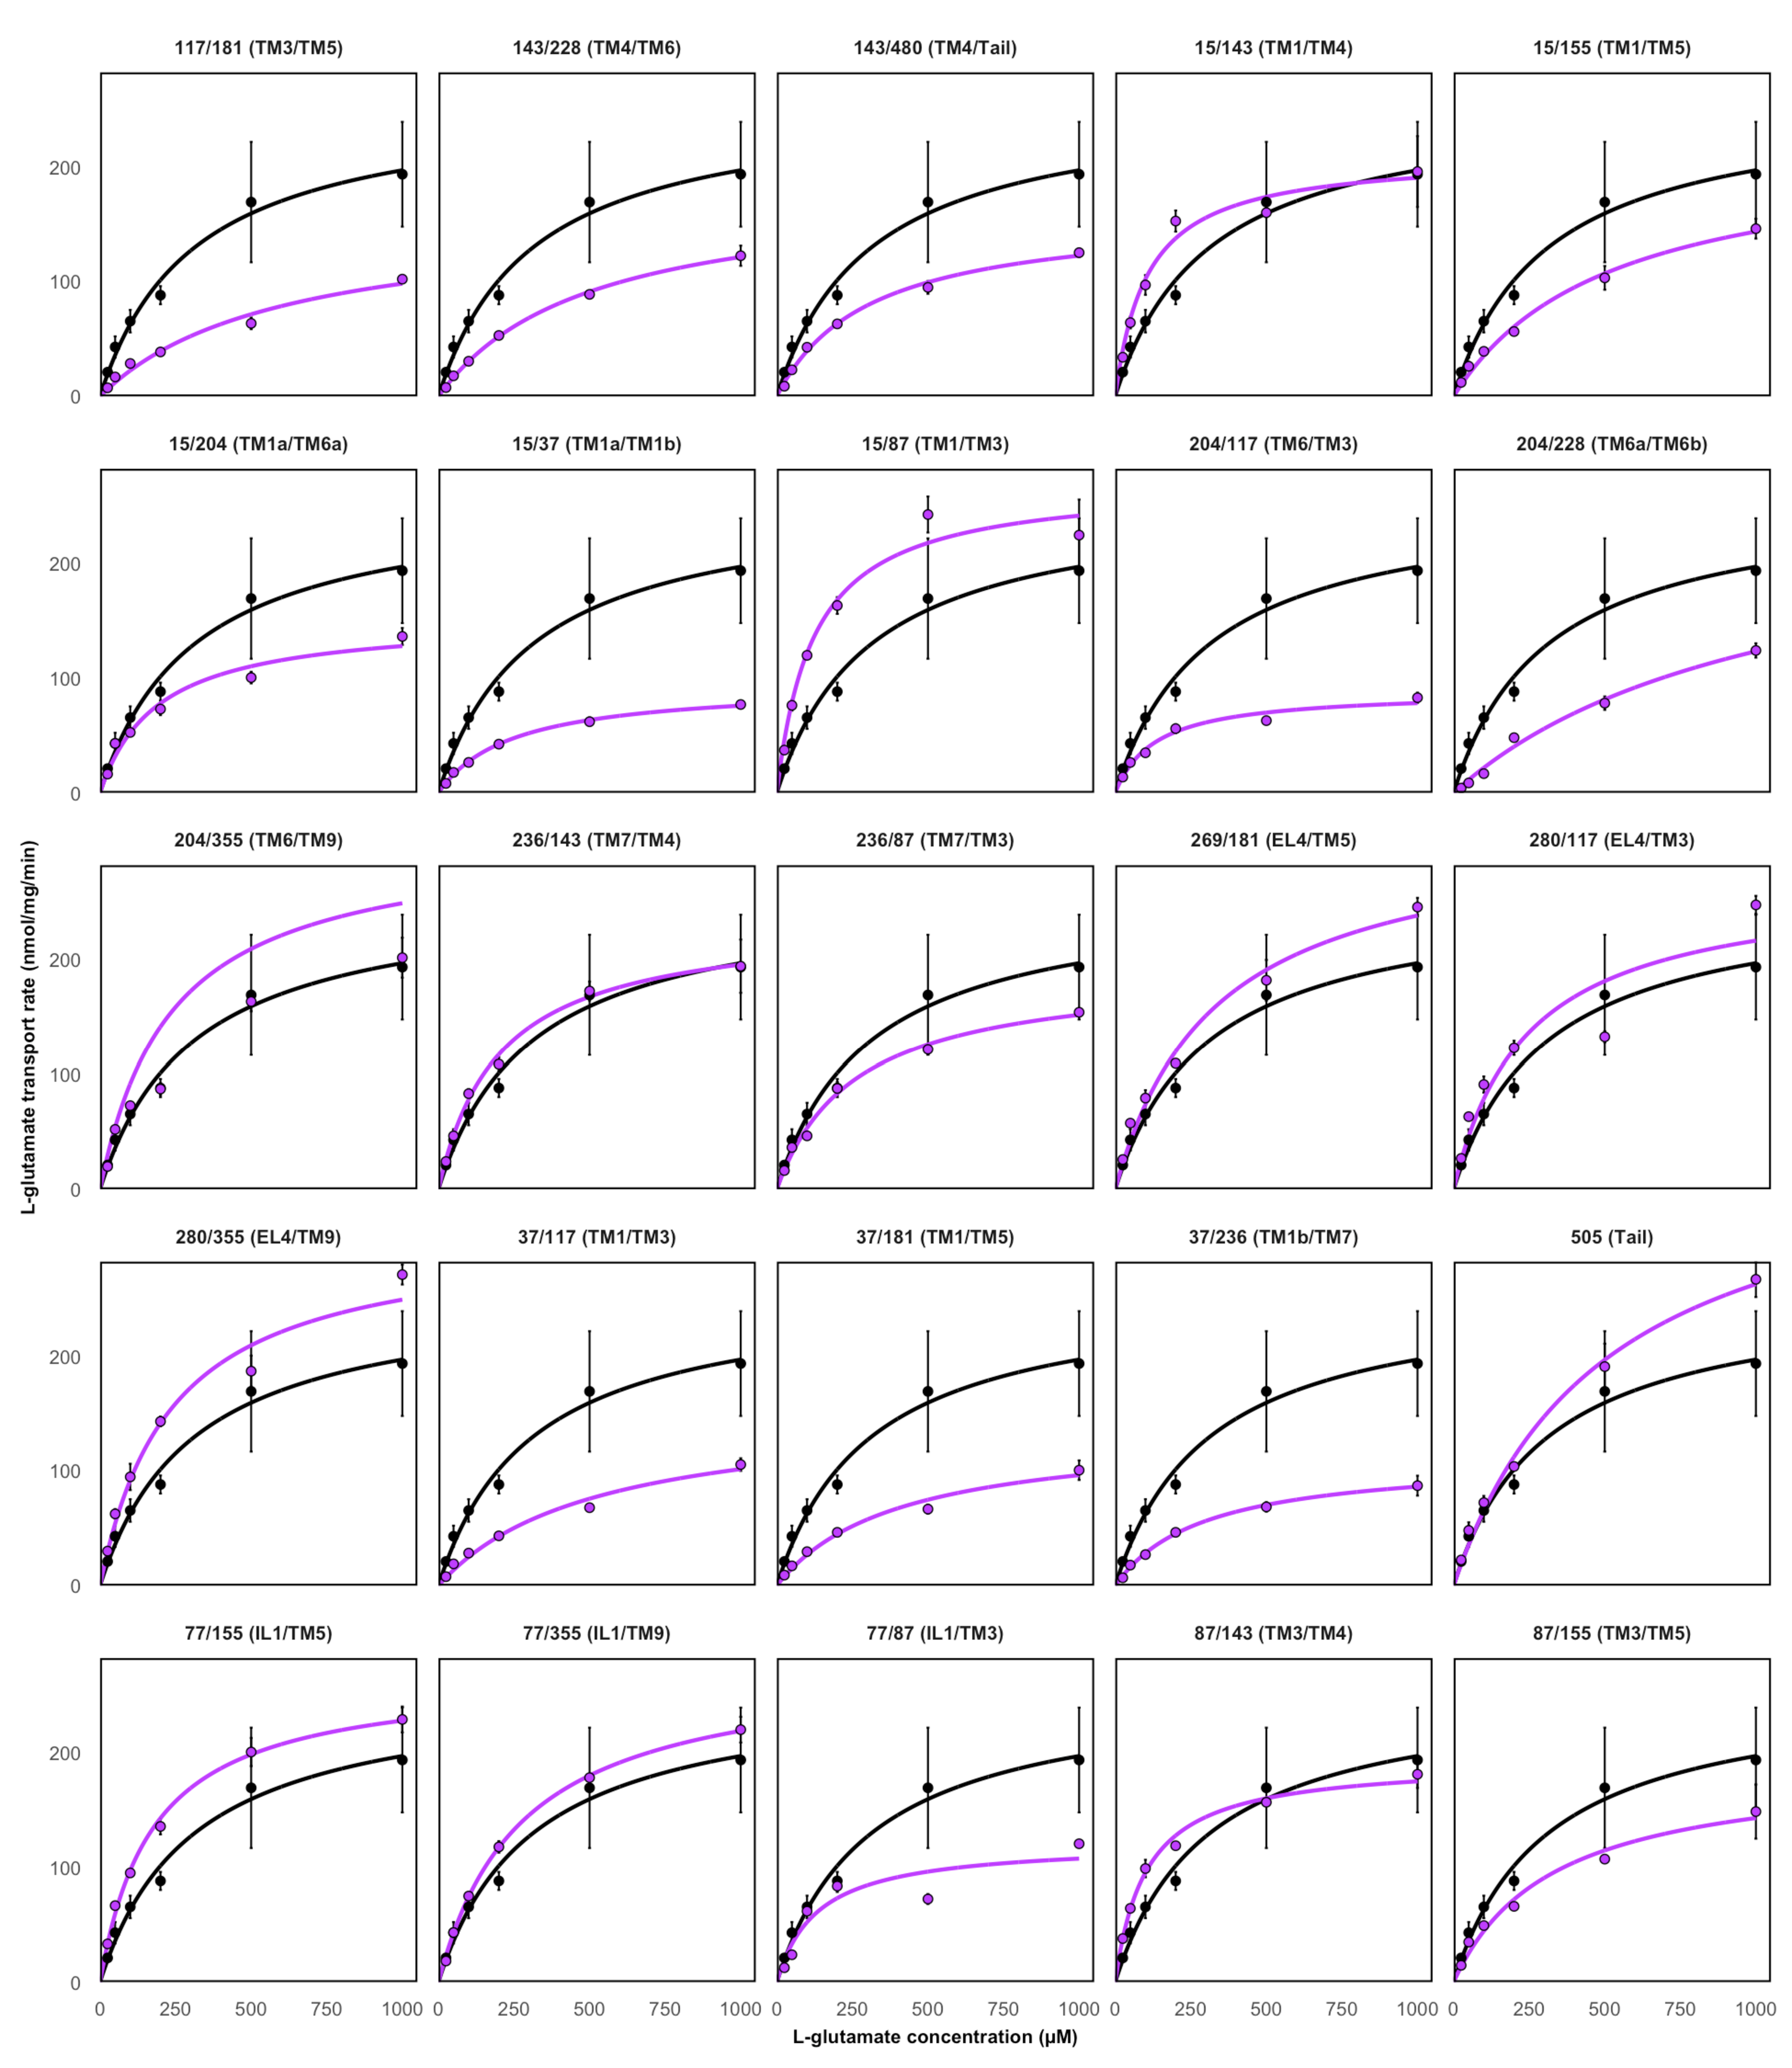
\includegraphics[width=5.5in]{Figures/gadc_supp_transport45.pdf}
\caption[Glutamate transport activity by GadC cysteine mutants.]{Glutamate transport activity by GadC cysteine mutants. All experiments executed in triplicate and baseline-normalized. Wildtype transport rate is shown in black. Error bars show the standard error of the mean.}
\label{fig:gadc_supp_transport}
\end{figure}

\begin{figure}[h]
\centering
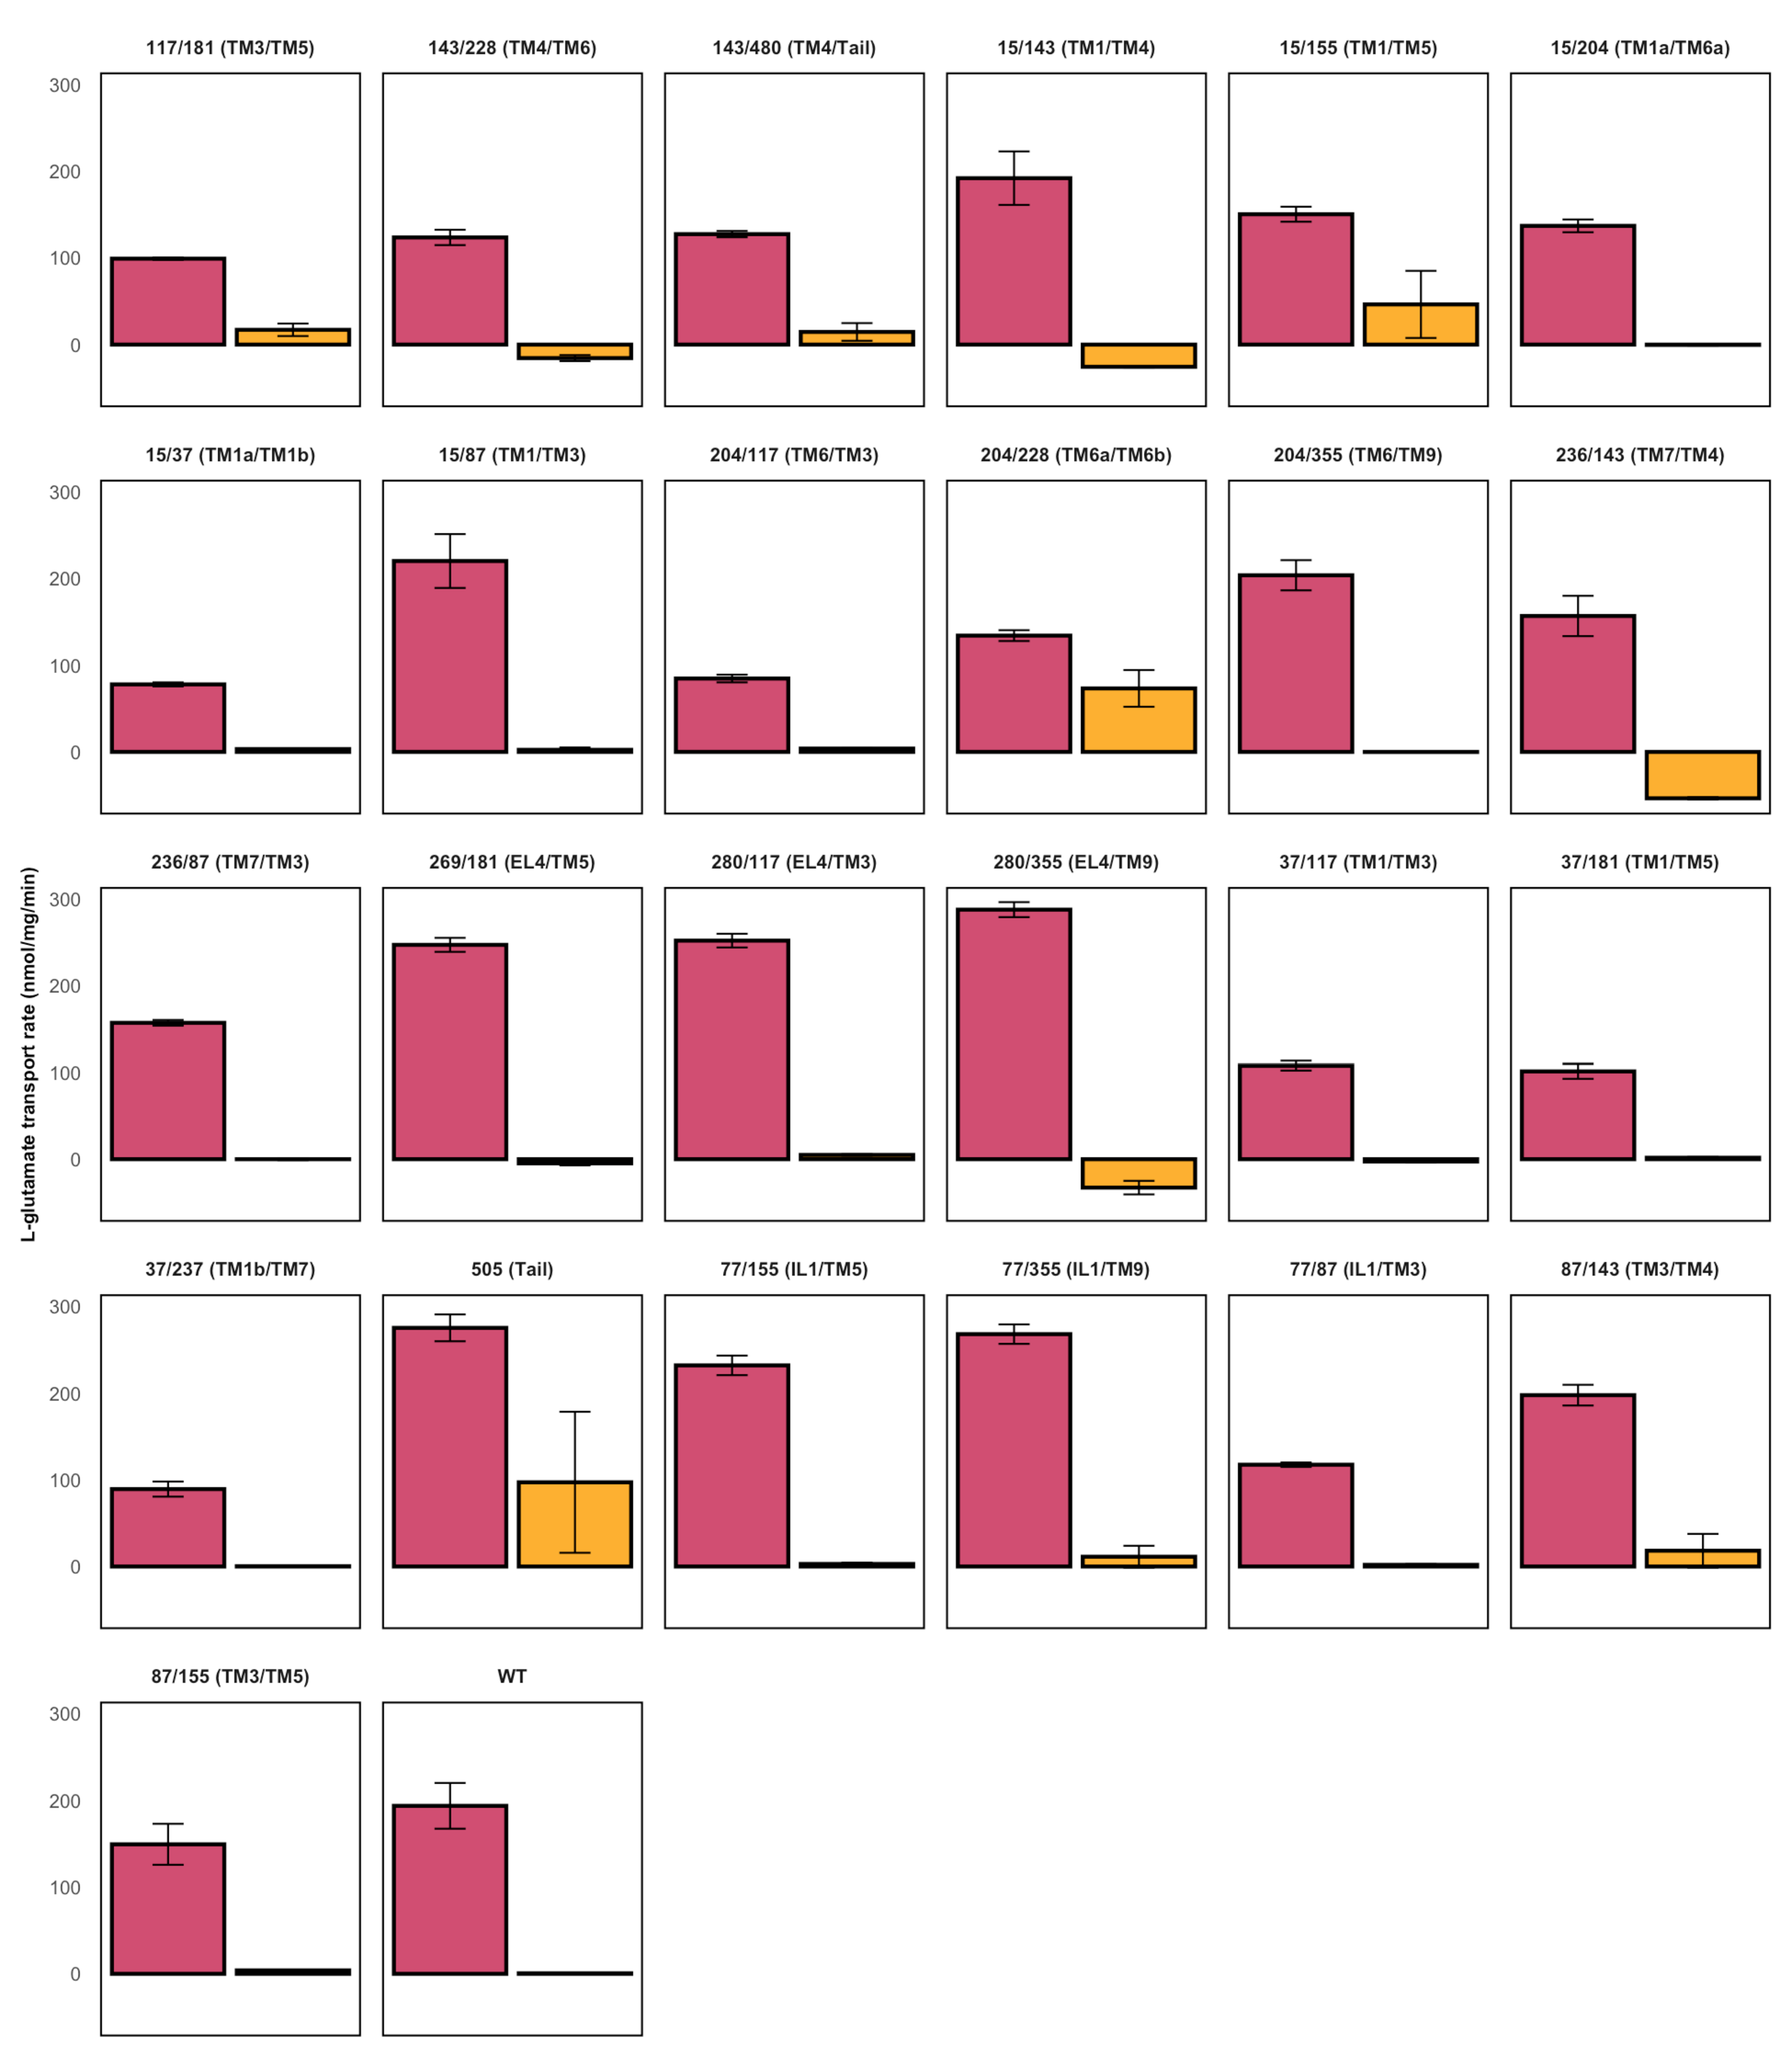
\includegraphics[width=5.5in]{Figures/gadc_supp_transport75.pdf}
\caption[pH-dependent inactivation of glutamate transport activity by GadC cysteine mutants.]{pH-dependent inactivation of glutamate transport activity by GadC cysteine mutants. Transport activity at pH 4.5 and 7.5 are shown in mauve and orange, respectively. All experiments executed in triplicate and baseline-normalized.}
\label{fig:gadc_supp_transport75}
\end{figure}

\begin{figure}[h]
\centering
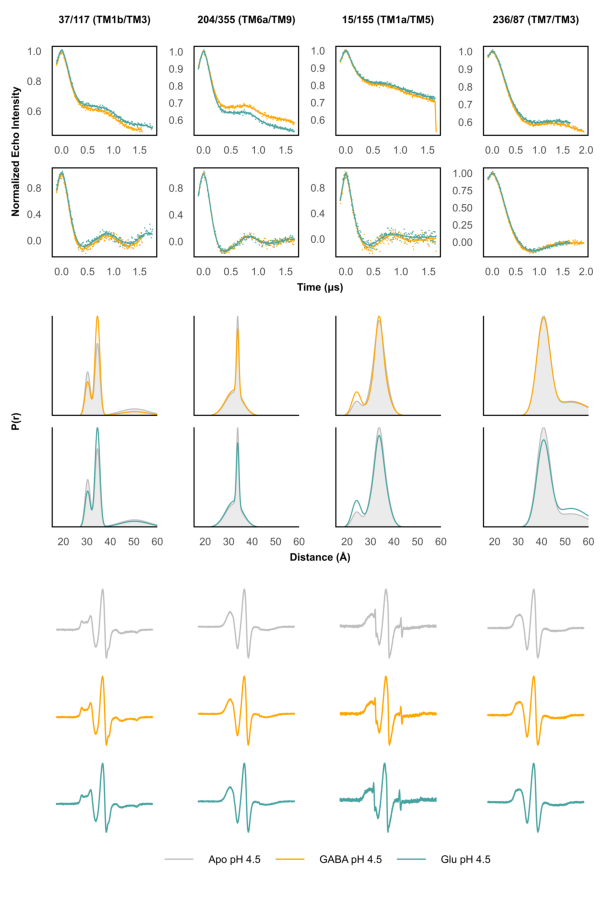
\includegraphics[width=5in]{Figures/gadc_supp_substrates.pdf}
\caption[Representative EPR pairs do not show evidence of large-scale substrate-dependent conformational changes in GadC.]{Representative EPR pairs do not show evidence of large-scale substrate-dependent conformational changes in GadC. Top: DEER traces prior to and following background-correction. Middle: DEER distance distributions at pH 4.5 with \SI{1}{mM} GABA (orange) or glutamate (teal). Apo distributions shown in grey. Bottom: continuous-wave EPR lineshapes with or without substrates.}
\label{fig:gadc_supp_substrates}
\end{figure}

\begin{figure}[h]
\centering
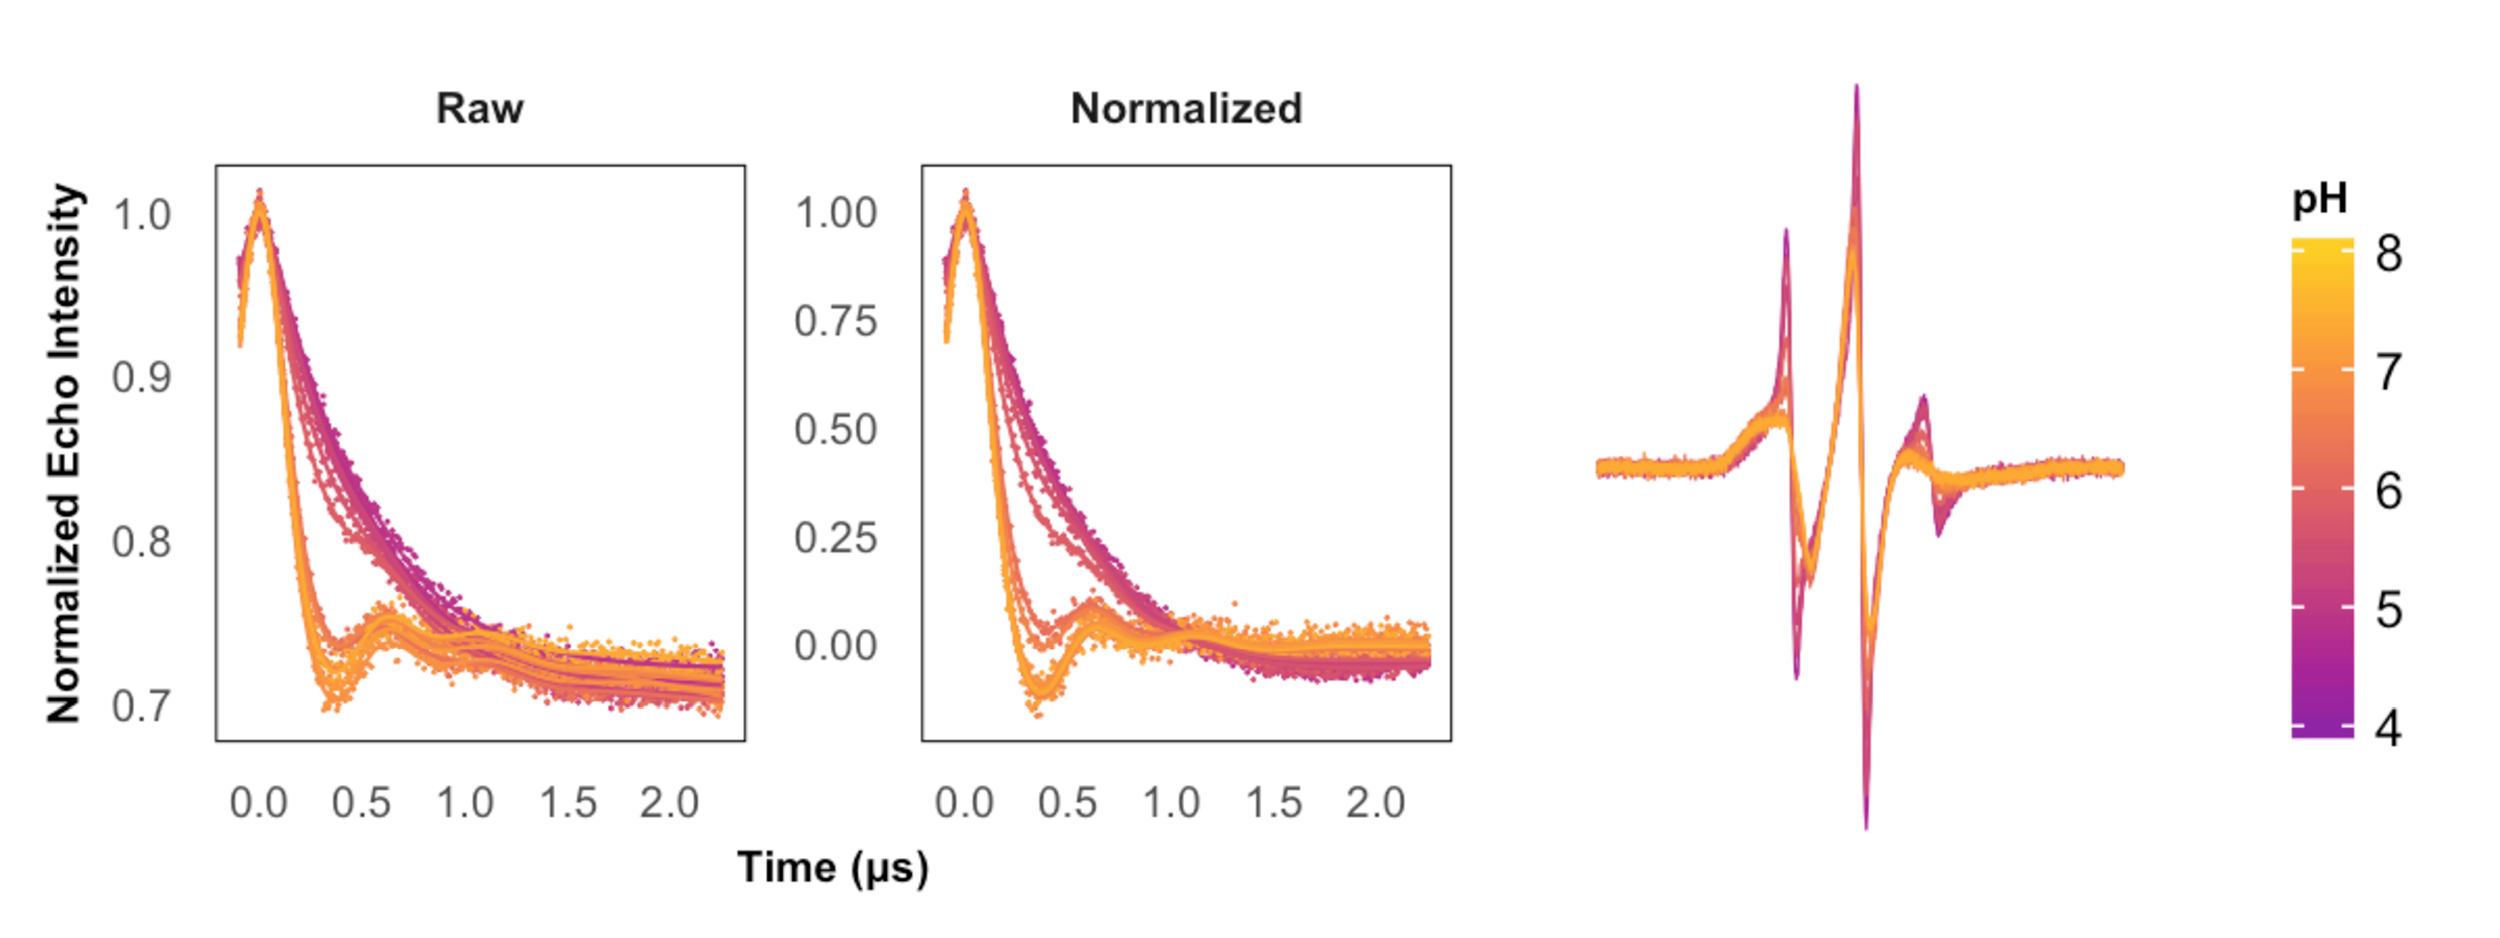
\includegraphics[width=5in]{Figures/gadc_supp_tail.pdf}
\caption[pH-dependent DEER data and continuous-wave EPR spectra of GadC 143/480.]{pH-dependent DEER data and continuous-wave EPR spectra of GadC 143/480.}
\label{fig:gadc_supp_tail}
\end{figure}

\begin{figure}[h]
\centering
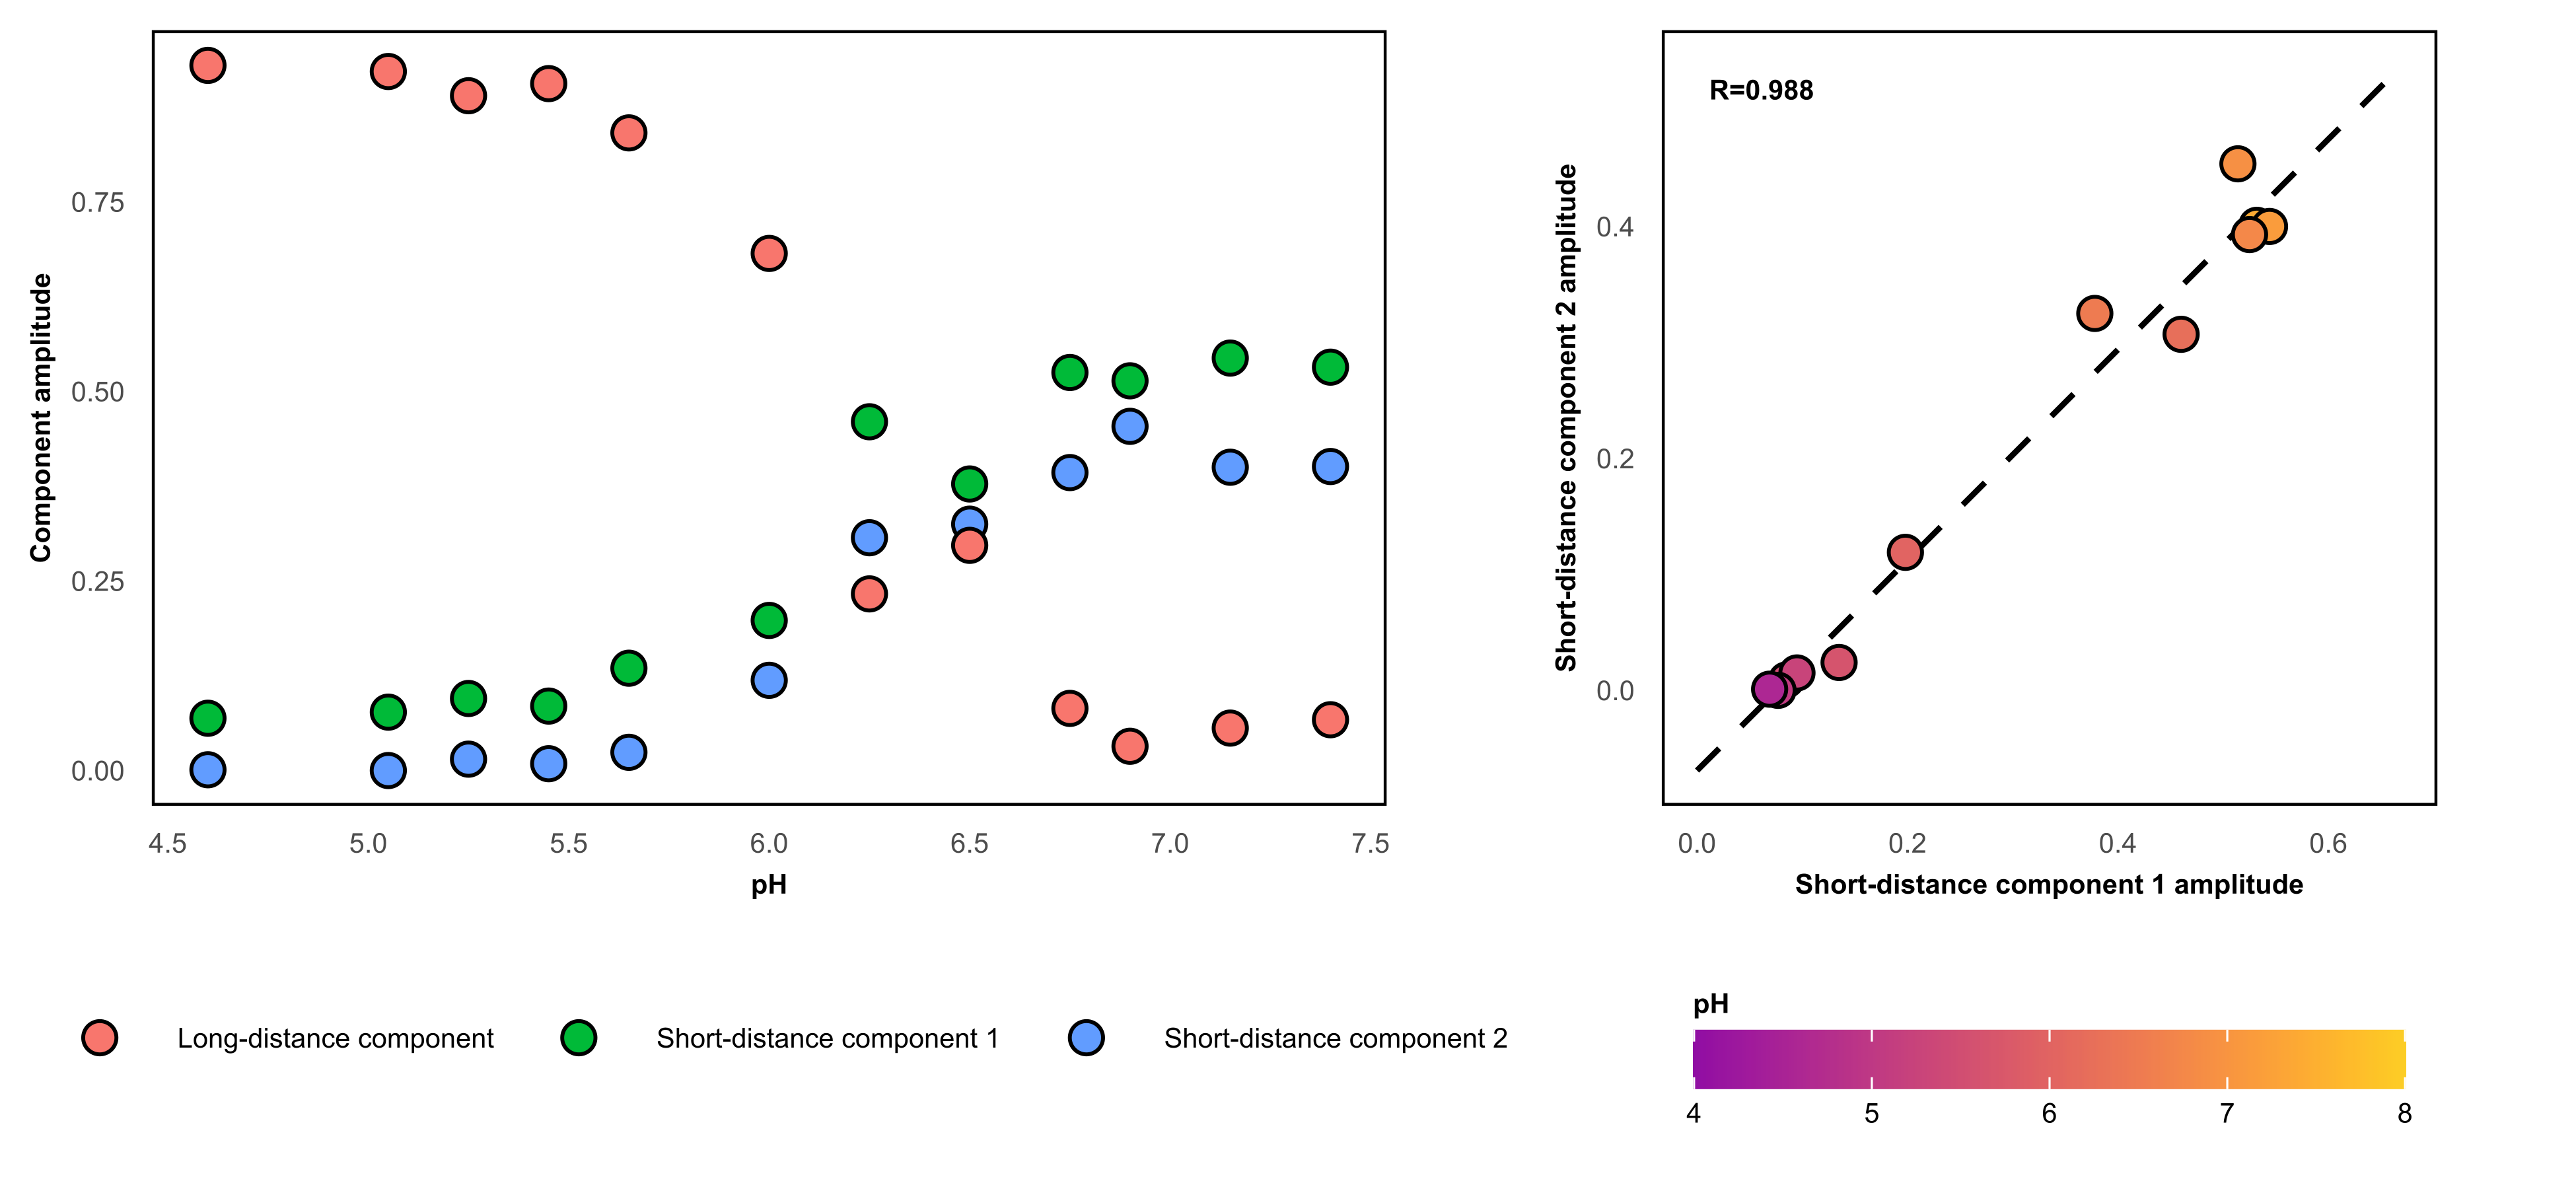
\includegraphics[width=6.5in]{Figures/gadc_supp_tail_rsq.png}
\caption[Correlation between short-distance DEER components in spin pair 143/480 during detachment of the tail.]{Correlation between short-distance DEER components in spin pair 143/480 during detachment of the tail.}
\label{fig:gadc_supp_tail_rsq}
\end{figure}

\begin{figure}[h]
\centering
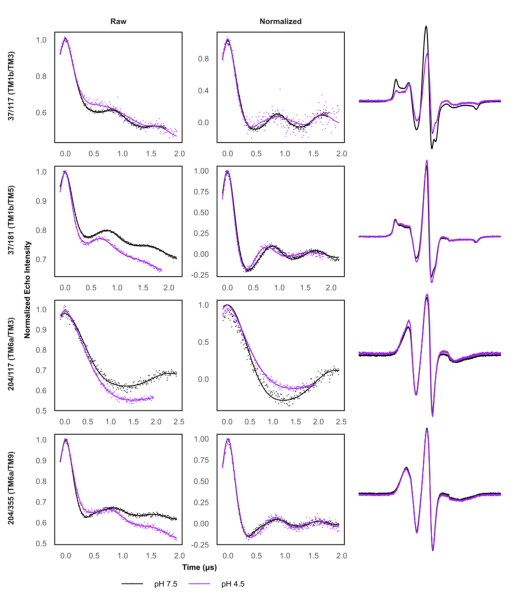
\includegraphics[width=3.5in]{Figures/gadc_supp_bundle_hash_extra.pdf}
\caption[DEER data and CW profiles of double-cysteine mutants labeled on both the bundle and scaffold domains on the extracellular side.]{DEER data and CW profiles of double-cysteine mutants labeled on both the bundle and scaffold domains on the extracellular side.}
\label{fig:gadc_supp_bundle_hash_extra}
\end{figure}

\begin{figure}[h]
\centering
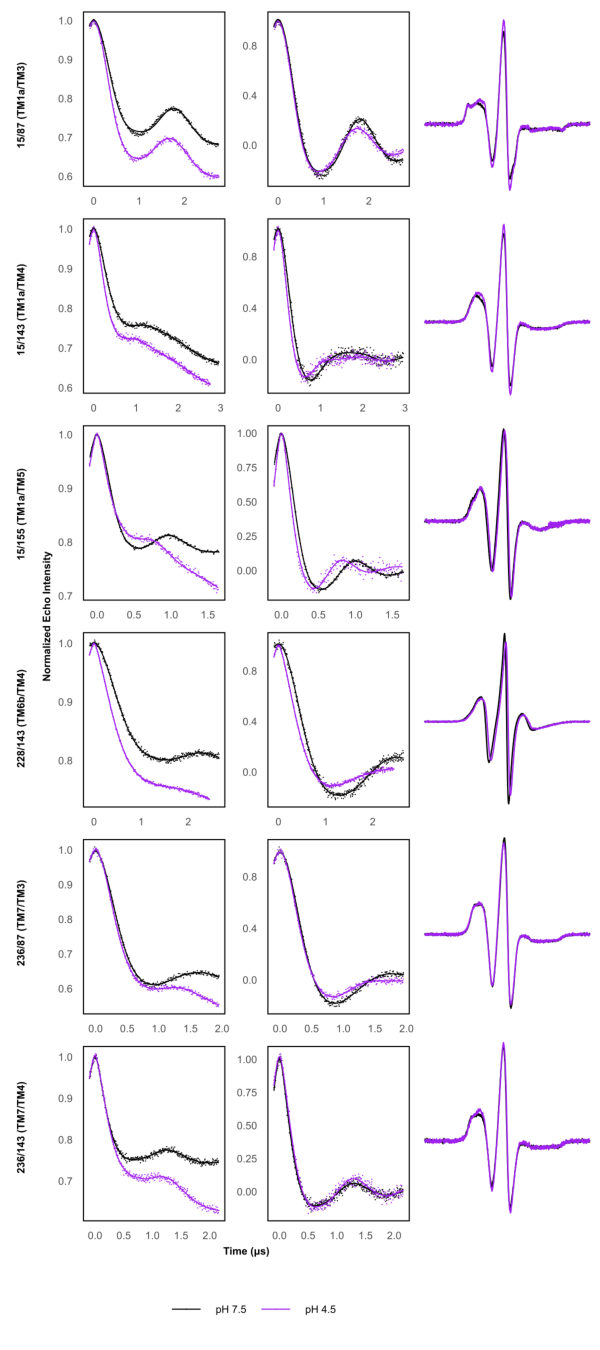
\includegraphics[width=3.5in]{Figures/gadc_supp_bundle_hash_intra.pdf}
\caption[DEER data and CW profiles of double-cysteine mutants labeled on both the bundle and scaffold domains on the intracellular side.]{DEER data and CW profiles of double-cysteine mutants labeled on both the bundle and scaffold domains on the intracellular side.}
\label{fig:gadc_supp_bundle_hash_intra}
\end{figure}


\begin{figure}[h]
\centering
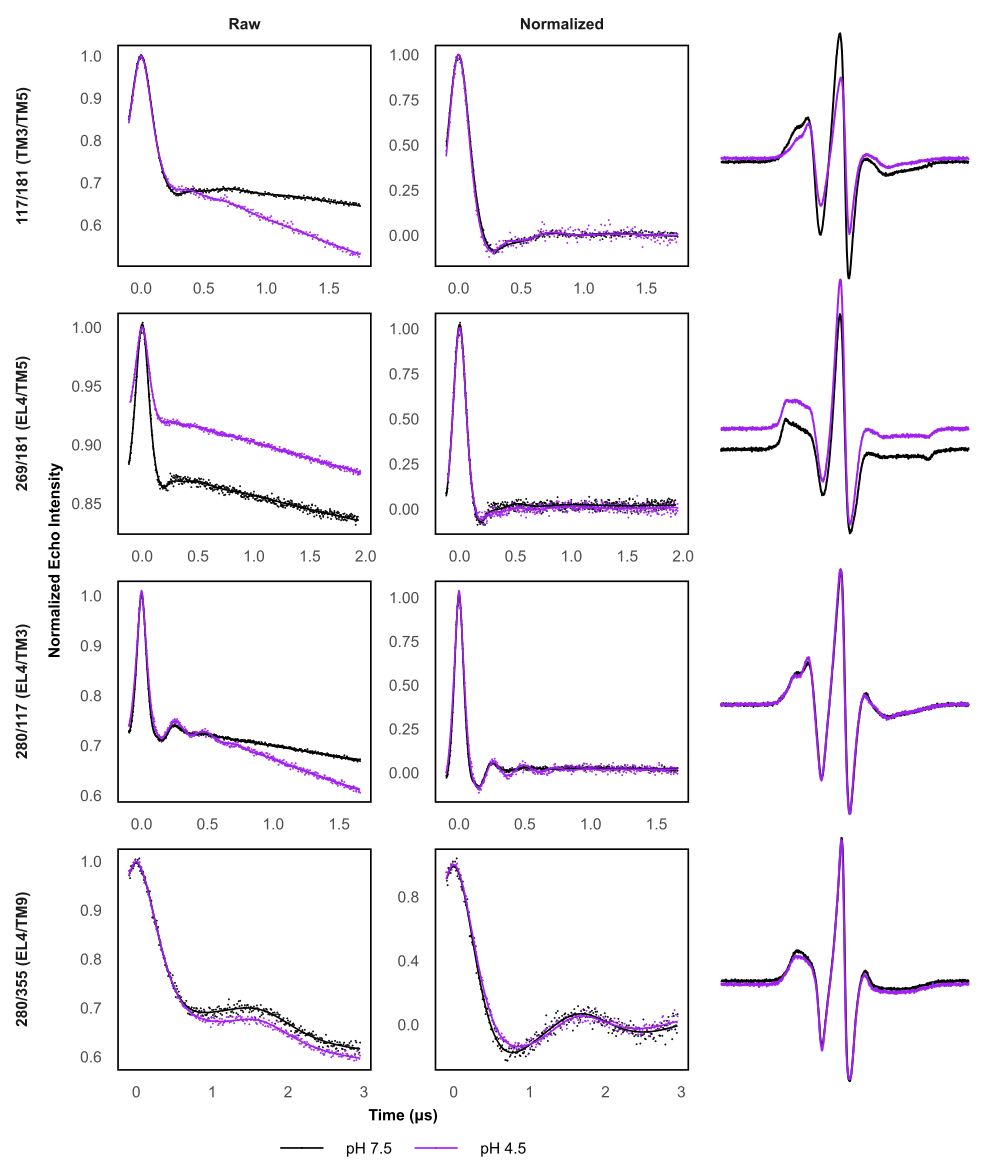
\includegraphics[width=3.5in]{Figures/gadc_supp_el4.png}
\caption[DEER data and CW profiles of double-cysteine mutants labeled in EL4 and the scaffold domain on the extracellular side.]{DEER data and CW profiles of double-cysteine mutants labeled in EL4 and the scaffold domain on the extracellular side.}
\label{fig:gadc_supp_el4}
\end{figure}

\begin{figure}[h]
\centering
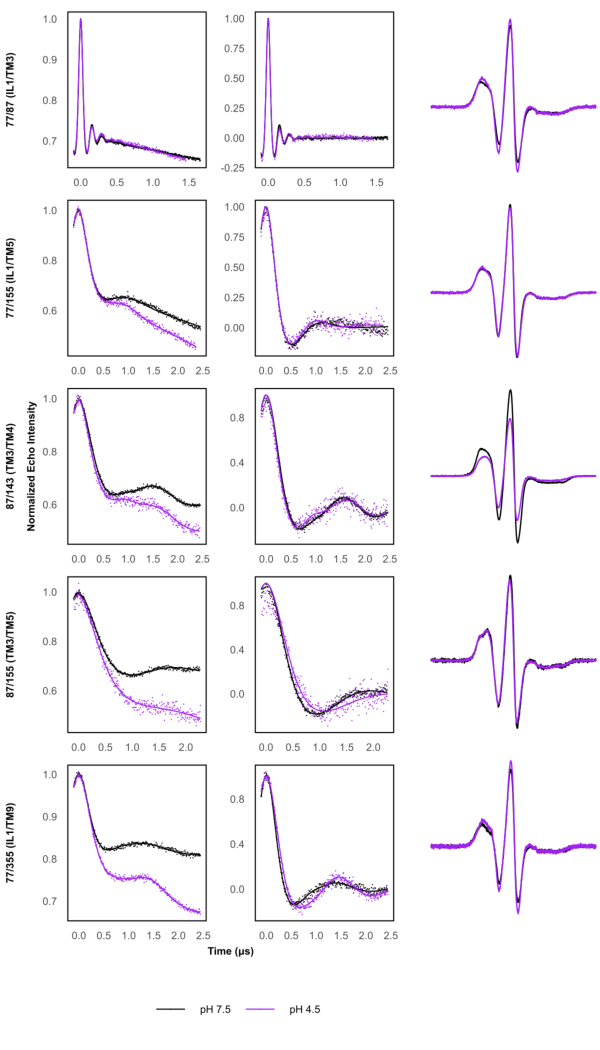
\includegraphics[width=3.5in]{Figures/gadc_supp_il1.pdf}
\caption[DEER data and CW profiles of double-cysteine mutants labeled in IL1 and the scaffold domain on the extracellular side.]{DEER data and CW profiles of double-cysteine mutants labeled in IL1 and the scaffold domain on the extracellular side.}
\label{fig:gadc_supp_il1}
\end{figure}

\begin{figure}[h]
\centering
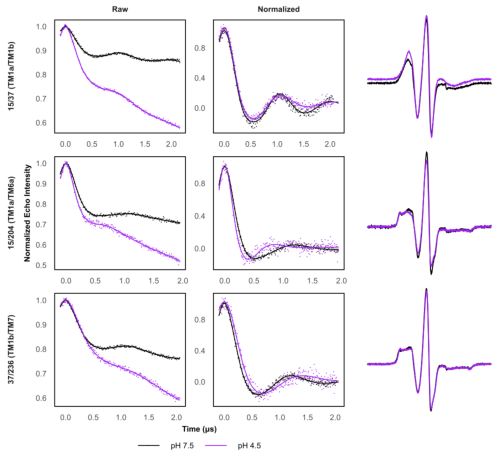
\includegraphics[width=3.5in]{Figures/gadc_supp_bundle_only.pdf}
\caption[DEER data and CW profiles of double-cysteine mutants labeled in the bundle domain.]{DEER data and CW profiles of double-cysteine mutants labeled in the bundle domain.}
\label{fig:gadc_supp_bundle_only}
\end{figure}

\begin{figure}[h]
\centering
\includegraphics[width=6.5in]{Figures/gadc_supp_models.pdf}
\caption[Positions of the transmembrane helices among the five best low pH (pink) and high pH (gray) models relative to crystal structure (shown in red, green, blue, and yellow for bundle domain, hash domain, gating helices and EL4, respectively).]{Positions of the transmembrane helices among the five best low pH (pink) and high pH (gray) models relative to crystal structure (shown in red, green, blue, and yellow for bundle domain, hash domain, gating helices and EL4, respectively).}
\label{fig:gadc_supp_models}
\end{figure}

\begin{figure}[h]
\centering
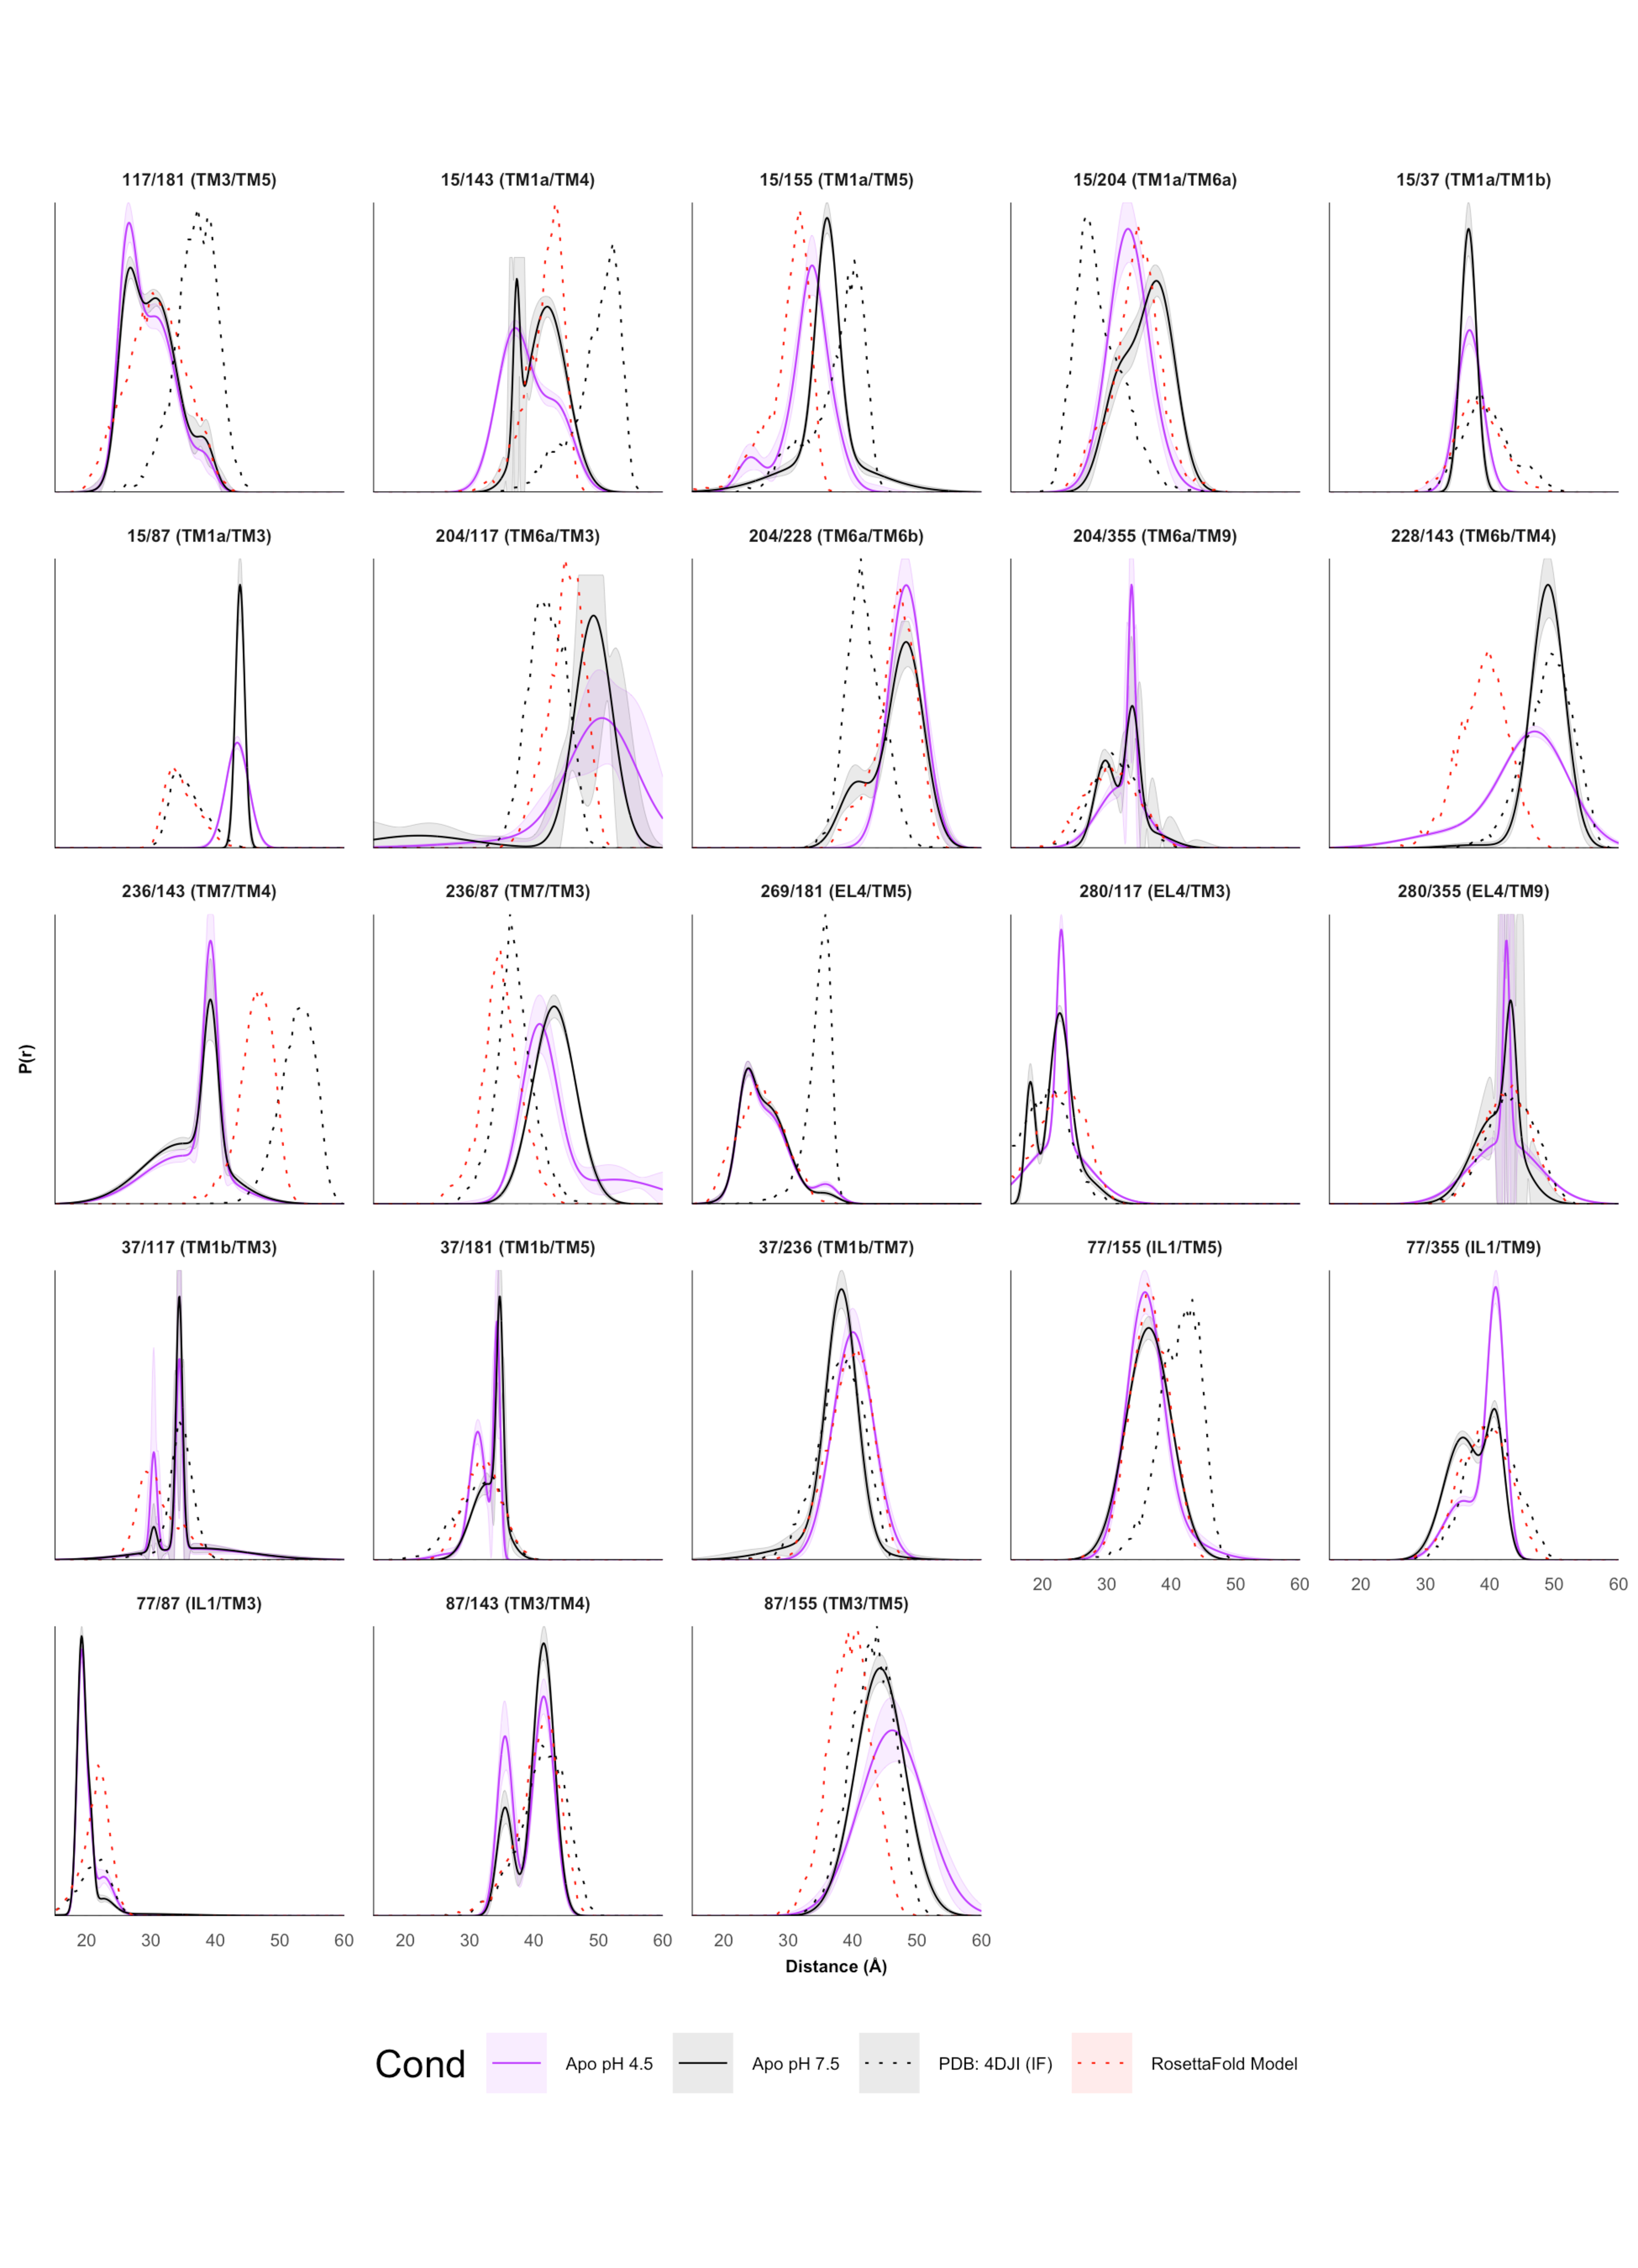
\includegraphics[width=5.5in]{Figures/gadc_supp_rosettafold.pdf}
\caption[Experimental DEER distance distributions measured in GadC and compared to a model generated \emph{de novo} using RosettaFold.]{Experimental DEER distance distributions measured in GadC and compared to a model generated \emph{de novo} using RosettaFold.}
\label{fig:gadc_supp_rosettafold}
\end{figure}